\chapter{Diseño e Implementación}

En este capítulo mostraremos los detalles del diseño y la implementacion de diferentes partes del proyecto.

\section{Gramáticas y frases}

La parte de la generación automática de frases y definición de gramáticas es la más relevante del proyecto y la que la diferencia del resto de juegos de similares caracteríticas. Por ello consideramos esencial mostrar su funcionamiento.

\begin{figure}
    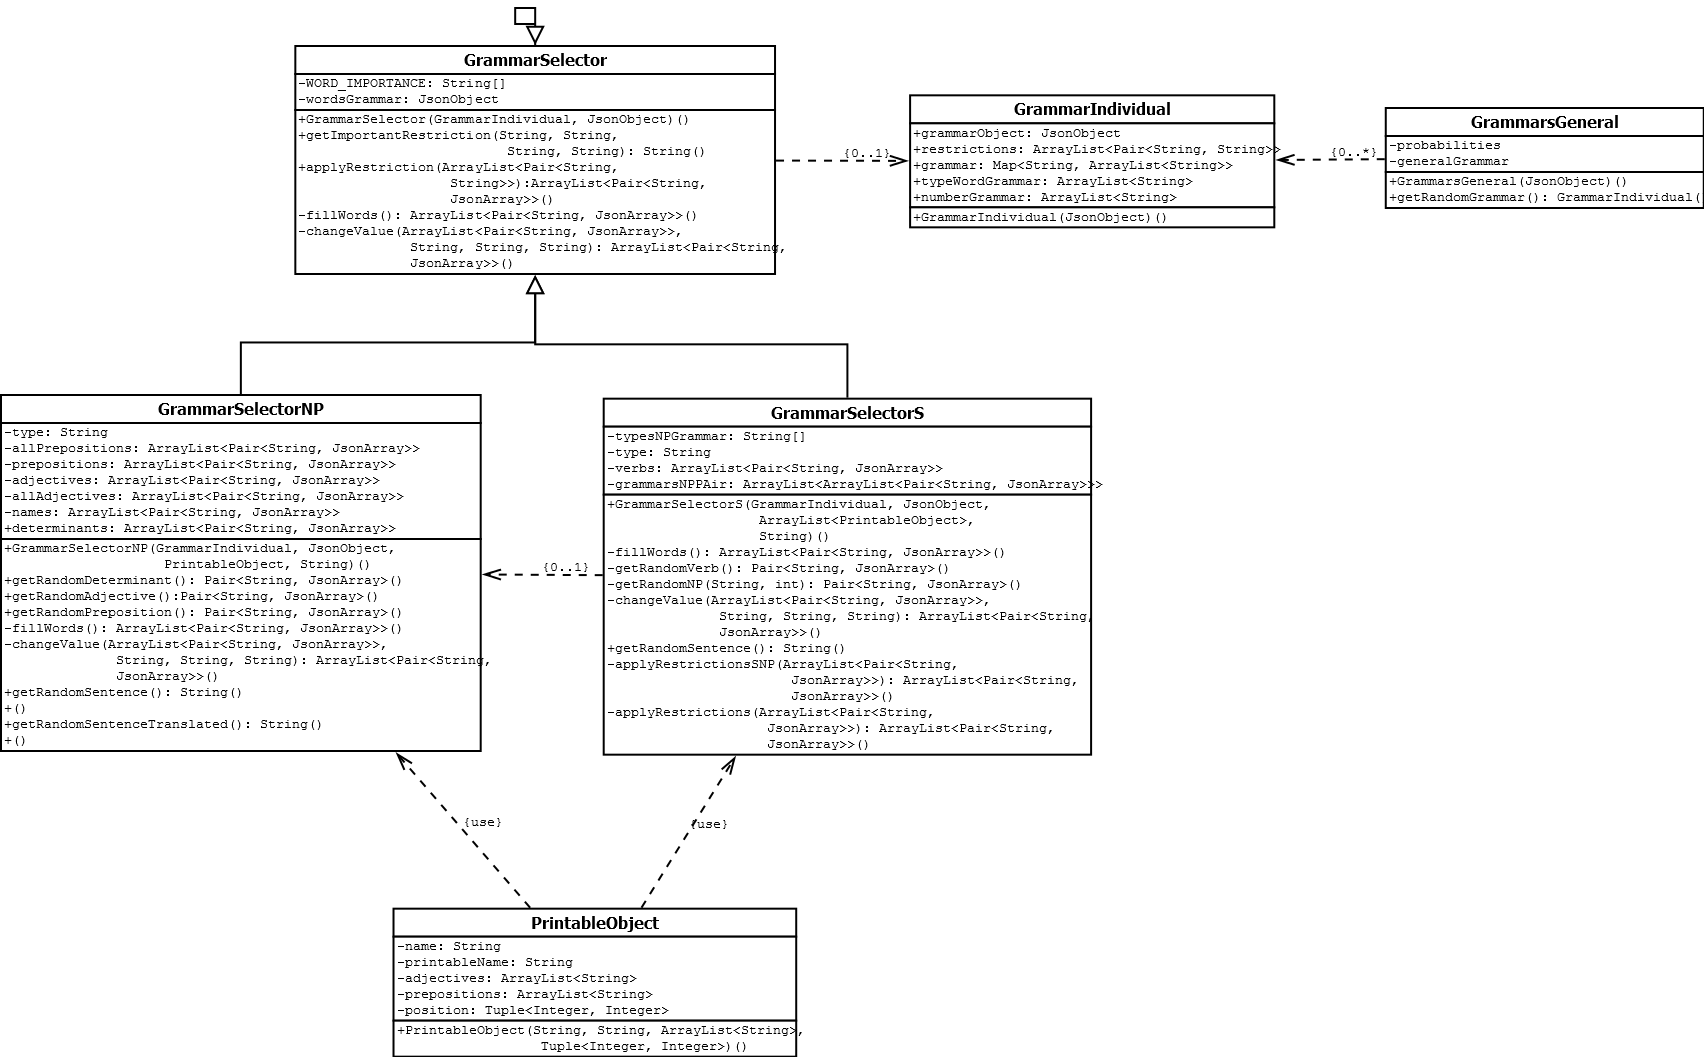
\includegraphics[width=\textwidth,height=\textheight,keepaspectratio,angle=90]{./img/grammarDiagram.png}
  \caption{Diagrama de clases de las gramáticas}
  \label{fig:clasesgramaticas}
\end{figure}

Tal y como se muestra en la figura ~\ref{clasesgramaticas}, la parte esencial de esta sección consta de seis clases, cuyo funcionamiento detalarremos un poco más adelante.

Cabe destacar que estas gramáticas, al igual que los diccionarios usados para cada uno de los idiomas, se obtienen en base a ficheros JSON dados.

\subsection{\textit{Input} de gramáticas y diccionario}

Tal y como hemos mencionado anteriormente, tanto las gramáticas como los diccionarios son archivos JSON que el usuario puede cambiar y que afectará al resultado de las frases generadas por el juego.

Para las gramáticas tenemos dos archivos por idioma. Uno de ellos son las gramáticas con las que creamos sintagmas nominales, mientras que las otras creamos frases usando, en su mayor parte, estos sintagmas nominales.

\subsubsection{Gramáticas: Sintagmas nominales}

Ejemplo de gramáticas de sigtagma nominal en inglés:

\begin{lstlisting}[style=json]
"DETADJN": {
    "GM_1": {
        "S": 
            [
            {"DET_1": ""}, 
            {"ADJ_1": ""}, 
            {"N_1": ""}
        ],
        "restrictions": [
            {"DET_1.num": "N_1.num"},
            {"N_1.num": "ADJ_1.num"}
        ]
    }
}
\end{lstlisting}

En estas gramáticas especificamos, primero, el nombre de la gramática (en este caso, DETADJN). Este nombre es usado por el programa y ayudará al usuario a entender el tipo de gramática o grupo de gramáticas que son.

El siguiente nombre es el nombre de la gramática en particular. No es usado en el programa, pero su uso es necesario para poder definir varias gramáticas sobre el mismo árbol (si queremos varias gramáticas de tipo DETADJN, necesitaremos que se especifiquen el nombre de cada una de ellas).

Luego viene el contenido relevante. Primero nos encontramos con \textit{S}, que es donde encontraremos la definición de la gramática en sí; y luego \textit{restrictions} que, como su nombre indica, es especificaremos las restricciones.

En la parte de la gramática tenemos, en este caso, \textit{DET\_1}, que es el primer determinante (y único) de la gramática, \textit{ADJ\_1}, el primer y único adjetivo que tiene dicha gramática y \textit{N\_1}, que es el nombre o sustantivo.
En las restricciones detallaremos las partes de la gramática que tienen que coincidir. En esta gramática solamente tenemos que el determinante, nombre y adjetivo tienen que ser iguales en número. Es decir, que ``the red swords'' no sería generada, sino que generaría ``the red sword''.

Este es un ejemplo en inglés, cuyas restricciones son más sencillas que en otros idiomas como el español o el gallego, donde el nombres, determinante y adjetivo no solamente tiene que coincidir número, pero también en género. Por este motivo, para generar el mismo tipo de gramática para estos idiomas, necesitaremos hacer lo siguiente:

\begin{lstlisting}[style=json]
"DETADJN": {
    "GM_1": {
        "S": 
            [
            {"DET_1": ""},
            {"N_1": ""},
            {"ADJ_1": ""}
        ],
        "restrictions": [
            {"DET_1.num": "N_1.num"},
            {"N_1.num": "ADJ_1.num"},
            {"DET_1.gen": "N_1.gen"},
            {"N_1.gen": "ADJ_1.gen"}
        ]
    }
}
\end{lstlisting}

Nótese que no solamente hemos añadido el género a las restricciones (para que no podamos generar frases como ``la espada rojo'' o ``el espada roja''), pero también hemos cambiado el orden del nombre y adjetivo para que se adapten a ambos idiomas. 

De esta manera podemos adaptar gramáticas a idiomas diferentes de una forma muy fácil y sin necesidad de tocar nada de código.

\subsubsection{Gramáticas: Frases}

Gramáticas para la generación de frases que usa las gramáticas de sintagma nominal: 

\begin{lstlisting}[style=json]
"ATTACK": {
	"S1": {
	    "S": [
	        {"SIMPLE_1": ""},
	        {"V_1": ""},
	        {"SIMPLE_2": ""},
	        {"SIMPLEPREP_1": ""}
	    ],
	    "restrictions": [
	        {"SIMPLE_1.num": "V_1.num"}
	    ]
	},
	"S2": {
	    "S": [
	        {"GENERAL_1": ""},
	        {"V_1": ""},
	        {"SIMPLE_2": ""},
	        {"SIMPLEPREP_1": ""}
	    ],
	    "restrictions": [
	        {"GENERAL_1.num": "V_1.num"}
	    ]
	}
}
\end{lstlisting}